\documentclass[class=article, crop=false]{standalone}
\usepackage{my_preamble}
\begin{document}
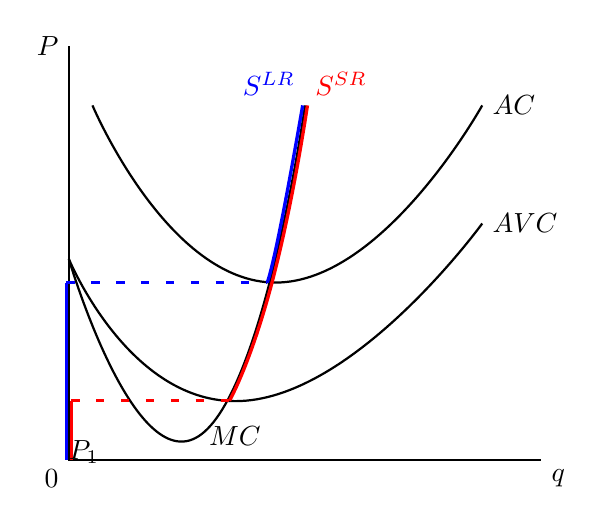
\begin{tikzpicture}[thick,font=\sffamily,scale=1.5]
	%axis and labels
	 \draw (0,3.5) node[left]{$P$} -- (0,0) node[below left] {$0$} 
	  -- (4,0) node[below right]{$q$};
	  
	%graphs	
	\draw[] plot [smooth, tension=1] coordinates {(0.2,3) (1.75,1.5) (3.5,3)}; %AC
	\draw[] plot [smooth, tension=1] coordinates {(0,1.7) (1.5,0.5) (3.5,2)}; %AVC
	\draw[] plot [smooth, tension=1] coordinates {(0,1.7) (1.1,0.2) (2,3)}; %MC
	
	%SR supply curve	
	\draw[very thick, red] (0.02,0) -- (0.02,0.5); %part 1
	\draw[very thick, red, loosely dashed] (0.02,0.5)--(1.36, 0.5); %part 2
	\draw[very thick, red] plot [smooth, tension=1] coordinates{(1.36, 0.5) (1.72,1.5) (2.02,3)}; %part 3

	%LR supply curve	
	\draw[very thick, blue] (-0.02,0) -- (-0.02,1.5); %part 1
	\draw[very thick, blue, loosely dashed] (-0.02,1.5)--(1.68, 1.5); %part 2
	\draw[very thick, blue] plot [smooth, tension=1] coordinates{(1.68,1.5) (1.795, 1.99) (1.98,3)}; %part 3

	%labelS
	\node[above right] at (2,3) {\textcolor{red}{$S^{SR}$}}; %SR supply label  
	\node[above left] at (2,3) {\textcolor{blue}{$S^{LR}$}}; %LR supply label  
	\node[right] at (3.5,3) {$AC$}; %AC label 
	\node[right] at (3.5,2) {$AVC$}; %AVC label
	\node[right] at (1.1,0.2) {$MC$}; %MC label
	
	%dotted lines
	%\draw[loosely dotted] (0,1) node[left]{$S_1$} -| node[pos=0.25,below=3mm] {}
  (1,0) node[below]{$P_1$}; %S1 and P1
	
\end{tikzpicture}
\end{document}